\section{试件热导率测试}
\subsection{测试方法选择}
进入测试方法界面,按\textcolor{red}{导热系数测量}按钮(见\figref{fig:exmp_kappa_chooseMethod})。同时,在每个测试实验里面,
按\textcolor{red}{切换方法}按钮,即可返回到选择测试方法界面(见\figref{fig:exmp_kappa_switchMethod})。
\begin{figure}[H]
	\centering
	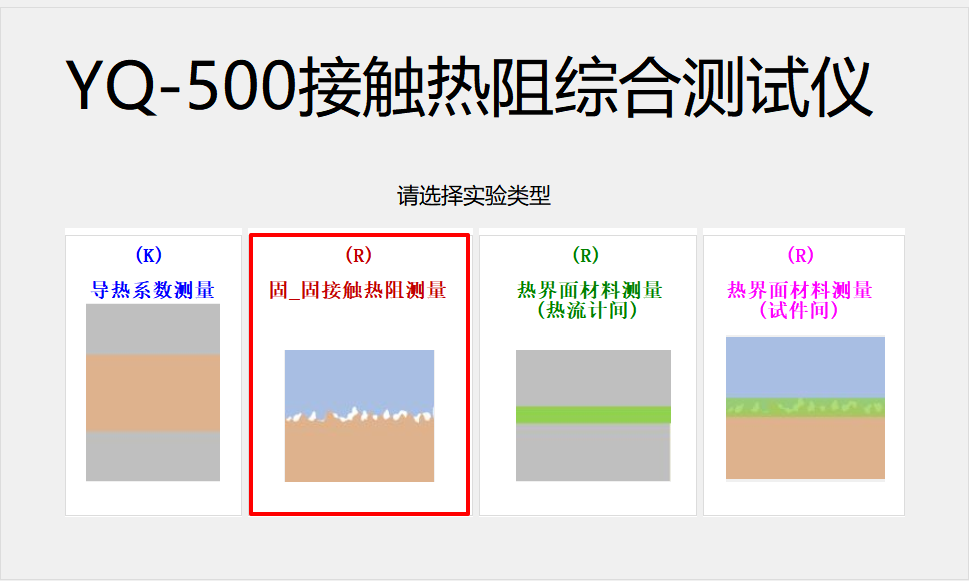
\includegraphics[width=1\textwidth]{example/KAPPA/chooseMethod.png}
	\caption{ 测试方法选择 \label{fig:exmp_kappa_chooseMethod}}
\end{figure}

\begin{figure}[H]
	\centering
	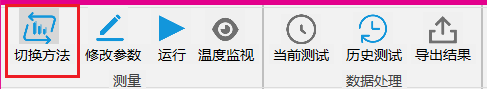
\includegraphics[width=1\textwidth]{example/KAPPA/switchMethod.png}
	\caption{ 切换方法 \label{fig:exmp_kappa_switchMethod}}
\end{figure}

\subsection{参数设置}
用户可根据实验条件,按\textcolor{red}{修改参数}按钮设置参数(见\figref{fig:exmp_kappa_changePara})。
\begin{figure}[H]
	\centering
	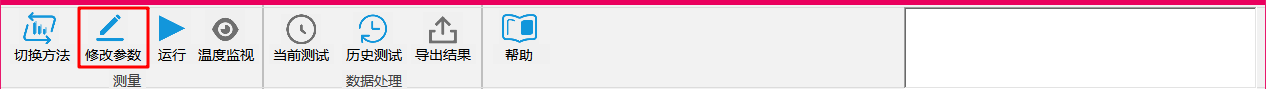
\includegraphics[width=1\textwidth]{example/KAPPA/changePara.png}
	\caption{ 修改参数 \label{fig:exmp_kappa_changePara}}
\end{figure}
在修改参数时,\textcolor{red}{高级用户}可以设置全部实验条件信息,而\textcolor{red}{普通用户}只可以设置试件的测温探头位置、通道编号、
样品截面积和加载压力等信息,设置完成按\textcolor{red}{确认参数}按钮保存(见\figref{fig:exmp_kappa_changeParaEnable})。
\begin{tips}{未启用的探头}
没有使用的测温探头,其位置和通道编号需要填入\textcolor{red}{*}作为参数。
同时,测温探头的位置参数应按照\textcolor{red}{现场测试的两相邻测温探头距离}要求严格填写。
\end{tips}
\begin{figure}[H]
	\centering
	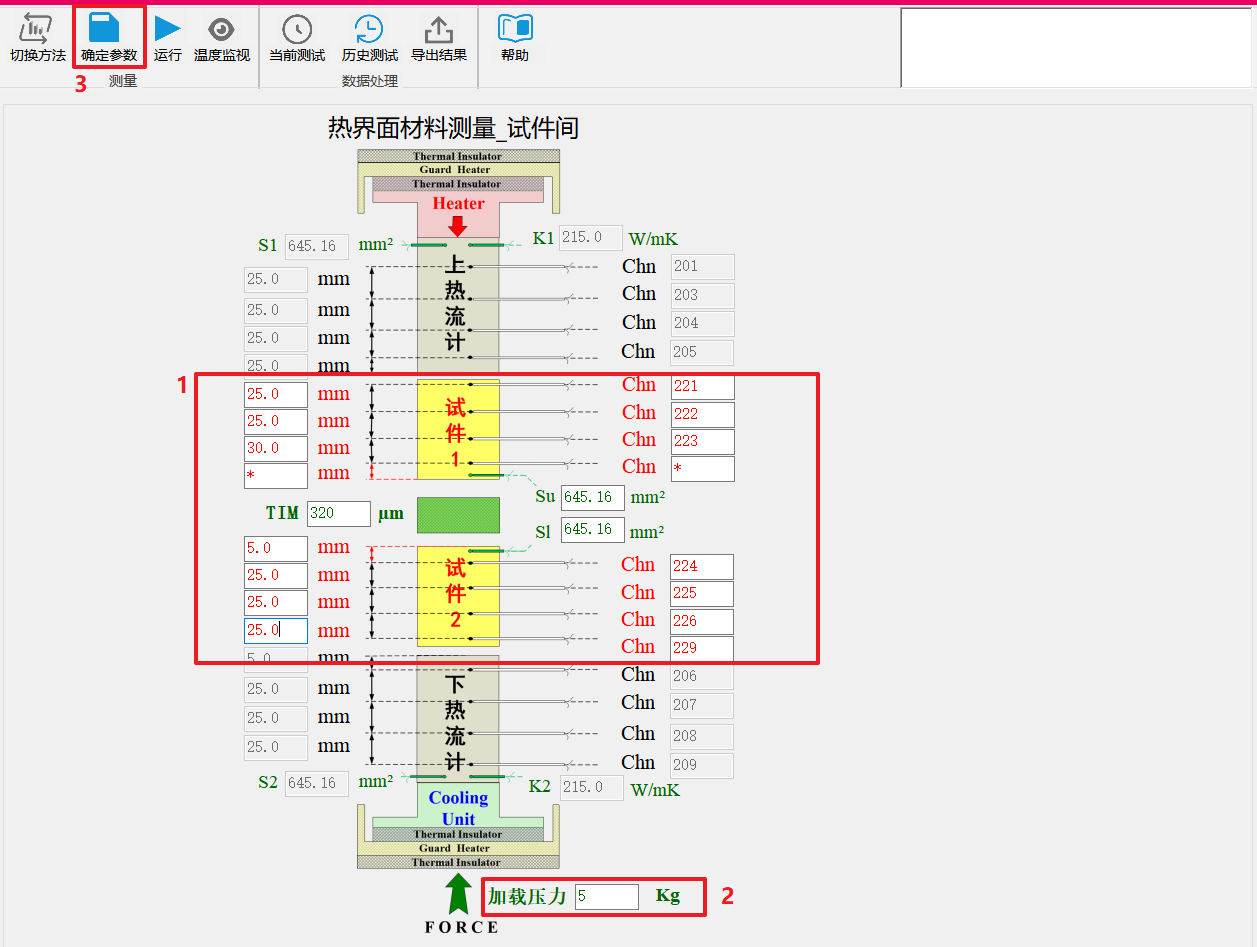
\includegraphics[width=0.9\textwidth]{example/KAPPA/changeParaEnable.png}
	\caption{ 确定参数修改 \label{fig:exmp_kappa_changeParaEnable}}
\end{figure}

\subsection{执行测试}
用户设计完参数后,按\textcolor{red}{运行}按钮即可开始实验测试(见\figref{fig:exmp_kappa_run})。
\begin{figure}[H]
	\centering
	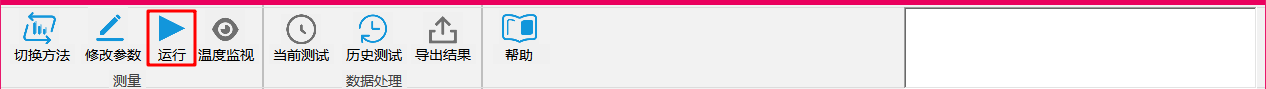
\includegraphics[width=1\textwidth]{example/KAPPA/run.png}
	\caption{ 运行 \label{fig:exmp_kappa_run}}
\end{figure}
在运行的时候,按\textcolor{red}{温度监控}按钮即可显示实时的探头温度信息见(\figref{fig:exmp_kappa_tempMirror})。
\begin{figure}[H]
	\centering
	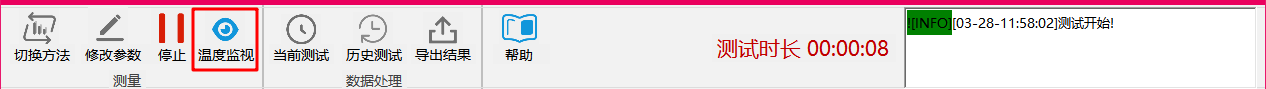
\includegraphics[width=1\textwidth]{example/KAPPA/tempMirror.png}
	\caption{ 温度监视图表 \label{fig:exmp_kappa_tempMirror}}
\end{figure}
\textcolor{red}{温度监控}可实时显示各测温探头温度,上部为各通道图例,可对其进行显示或隐藏,
左下角可设置\textcolor{red}{实时/全局显示}和\textcolor{red}{纵轴放大},右上角按\textcolor{red}{隐藏图表}按钮可对其隐藏。
特别的,勾选\textcolor{red}{纵轴放大},再用鼠标按压左键框选,可实现纵轴放大,若想恢复原始范围,
点击左上角滚轴\textcolor{red}{'-'}即可;鼠标指向温度线时,可捕获其通道编号、采集时间和温度信息(见\figref{fig:exmp_kappa_chartEdit})。\\
\begin{figure}[H]
	\centering
	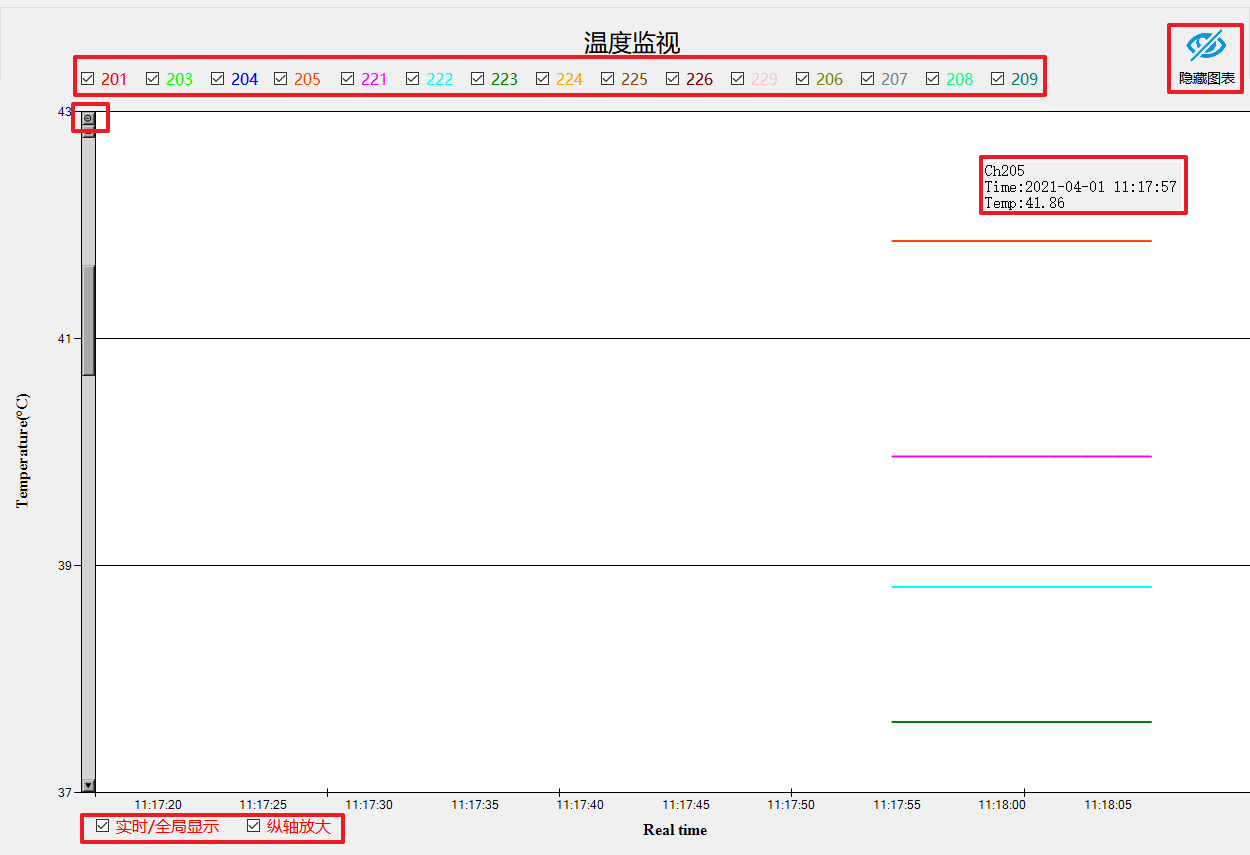
\includegraphics[width=0.9\textwidth]{example/KAPPA/chartEdit.png}
	\caption{ 图表显示设置 \label{fig:exmp_kappa_chartEdit}}
\end{figure}

\subsection{获取测试结果}
	当温度曲线稳定,按\textcolor{red}{当前测试}按钮即可自动求得结果(见\figref{fig:exmp_kappa_currentTest})。
\begin{tips}{结果计算}
	软件通过数采仪获取一定数量的数据才可以计算,同时为了保证实验的准确性,应等待温度相对稳定在某一范围
再点击\textcolor{red}{当前测试}按钮计算结果。
\end{tips}
\begin{figure}[H]
	\centering
	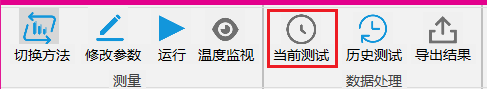
\includegraphics[width=0.9\textwidth]{example/KAPPA/currentTest.png}
	\caption{ 当前测试结果 \label{fig:exmp_kappa_currentTest}}
\end{figure}
软件可处理历史采集的实验数据,默认历史数据保存在安装根目录下\textcolor{red}{AutoSave}的文件中,
选择\textcolor{red}{(.rst)类型}文件,即可自动计算实验结果(见\figref{fig:exmp_kappa_historicalTest})。得到实验结果后,
按\textcolor{red}{导出结果}按钮,将实验结果以图片形式保存(见\figref{fig:exmp_kappa_exportResult})。
\begin{figure}[H]
	\centering
	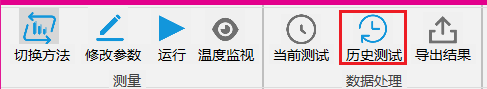
\includegraphics[width=0.9\textwidth]{example/KAPPA/historicalTest.png}
	\caption{ 历史测试结果 \label{fig:exmp_kappa_historicalTest}}
\end{figure}

\begin{figure}[H]
	\centering
	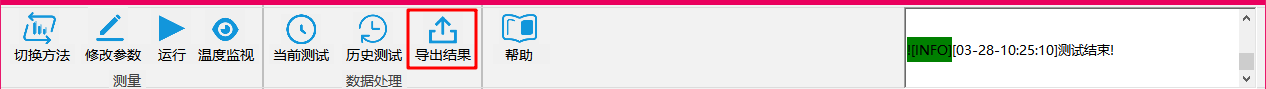
\includegraphics[width=0.9\textwidth]{example/KAPPA/exportResult.png}
	\caption{ 导出测试结果 \label{fig:exmp_kappa_exportResult}}
\end{figure}